% Chapter 2

\chapter{Fundamentação Teórica}\label{chap:background}
Ao longo deste capítulo é apresentado o embasamento teórico do projeto,
o qual dispõe de pesquisas já realizadas por outros autores sobre os temas
propostos e os conceitos que servirão de base para o desenvolvimento do
atual trabalho.

\section{Área de Negocio}\label{sec:business}
\subsection{Gestão do Conhecimento}

Em tradução de \cite[p. 4]{2014:Becerra} a Gestão de Conhecimento,
em inglês \emph{Knowledge Management} ou \emph{KM}, pode ser definida
como "fazer oque for necessário para tirar o máximo de proveito do
recursos de conhecimento disponíveis". A Gestão de Conhecimento pode
ser aplicada para indivíduos, porem vem ganhando atenção por parte
das organizações, pois é vista como uma disciplina que promove
a criação, compartilhamento e aproveitamento do conhecimento.

Já em tradução de \citep[p. 26]{2007:Awad} a Gestão de Conhecimento
é um modelo de negócios interdisciplinar emergente, que possui
o conhecimento como sendo o centro da estrutura da organização.
Possuindo raízes em varias disciplinas, incluindo economia empresarial,
psicologia e gestão da informação, e envolvendo pessoas, tecnologias e
processos.

Conforme o mesmo autor, a Gestão de Conhecimento também pode ser
o processo de capturar e fazer uso do conhecimento coletivo da organização,
sendo separado em dois tipos, o conhecimento explicito, que é documentado
em papel ou em bases de dados, e o conhecimento tácito, que existe
somente na mente dos indivíduos.

Seguindo a definição proposta por \cite{2014:Becerra}, a
Gestão de Conhecimento possui foco em organizar e tornar o
conhecimento disponível, onde e quando for necessário.
Tendo sua enfeasse em conhecimentos que já foram reconhecidos e
articulados de alguma forma, incluindo o conhecimento sobre os
processos de uma organização, procedimentos, propriedade intelectual,
documentação de boas práticas, previsões, lições aprendidas, e soluções
para problemas recorrentes.

Aos poucos a Gestão de Conhecimento também vem abordando a enfase sobre documentar
e organizar o conhecimento que muitas vezes só reside dentro das mentes
dos colaboradores mais experientes da organização.

\subsection{Repositórios Institucionais}

Em tradução livre de \cite{LYNCH:2003} repositórios institucionais podem
ser definidos como sendo um conjunto de serviços que a universidade pode
oferecer aos seus membros, visando o gerenciamento e disseminação dos matérias
digitais produzidos tanto pela instituição quanto pelos membros de sua comunidade.

Já em tradução de \cite{2015:Callicott} a iniciativa de repositórios institucionais
consiste em um conjunto de serviços que possuem o objetivo suportar a preservação,
organização e acesso aos conhecimentos produzidos pela instituição. No sentido de
infraestrutura de software, são desenvolvidos para solucionar alguns dos problemas
que a comunicação acadêmica enfrenta na era digital, oferecendo a possibilidade
de publicação imediata, preservação de longo prazo e acesso global as publicações.

Conforme o mesmo autor, a ideia geral de repositório institucional surgiu com o
lançamento do repositório de disciplinas especificas arXiv em 1991. Em seu
lançamento a comunicação eletrônica de literatura acadêmica foi rapidamente
adotada por físicos, e desde então expandiu-se para outras areas correlatas
da física e matemática, hospedando mais de um milhão de \emph{e-prints}.

No inicio dos anos 2000, a ideia publicação imediata e aberta em
repositório disciplinares começou a ser popularizada e aplicada a nível
institucional. Em seguida em 2002, houve o lançamento da primeira versão
oficial do \emph{software open source} DSpace, junto a publicação da
\emph{Scholarly Publishing and Academic Resources Coalition} (SPARC),
e do paper \emph{The Case for Institutional Repositories} escrito por
Raym Crow.

Conforme \cite{2015:Callicott}, este dois eventos serviram como base
para \emph{softwares} amplamente acessíveis para repositórios institucionais,
além de vincular a ideia de que repositórios institucionais atuam
sobre a visibilidade e prestigio da instituição.

\subsection{Padrão Dublin Core para metadados descritivos}

Em tradução livre de \cite{2003:Caplan}
o padrão \emph{Dublin Core Metadata Element Set} ou somente \emph{Dublin Core}
pode ser definido como um esquema de propósito geral, utilizado para a descrição
de recursos e objetos na internet. O padrão consiste em um conjunto de 50
elementos, contendo ao menos um identificador e uma descrição de sua definição.

Já em tradução de \cite{2018:Banerjee} a história do padrão Dublin Core
remonta a segunda edição da \emph{International WWW Conference} em 1994.
Surgindo de uma discussão sobre a dificuldade existente no período em
encontrar materiais presentes na internet.

A partir desta discussão,
em 1995 em Dublin, Ohio, a OCLC (\emph{Online Computer Library Center}) e a
NCSA (\emph{National Center of Supercomputers Applications}) lideraram
em conjunto um \emph{workshop} que foi chamado de \emph{OCLC/NCSA Metadata Workshop},
tendo como objetivo decidir quais elementos seriam necessários para
promover a melhor encontrabilidade de documentos na internet, explorar
soluções sobre como criar mecanismos que seriam flexíveis para publicações
realizadas na internet no passado, presente e futuro, e como promover
que tais soluções sejam utilizadas caso já existam.

Neste encontro, os participantes entraram em acordo sobre um conjunto
elementos descritivos, dos quais 50 destes termos poderiam ser
virtualmente aplicados a qualquer recurso presente na internet até
o momento. Destes 50 termos, surgiu a iniciativa do padrão Dublin Core.

\begin{table}[H]
    \captionsetup{justification=centering}
    \caption{Exemplo de elementos do Dublin Core}
    \label{table:dublin-core-element-exemple}
    \centering
    \resizebox{1.0\textwidth}{!}{% 
        \begin{tabular}{|p{3cm}|p{14cm}|}
            \hline
            \textbf{Identificador} & \textbf{Definição}                                                     \\ \hline
            \emph{Title}           & Nome dado ao recurso.                                                  \\ \hline
            \emph{Creator}         & Entidade responsável pela criação do conteúdo do recurso.              \\ \hline
            \emph{Subject}         & Assunto do conteúdo do recurso.                                        \\ \hline
            \emph{Description}     & Descrição do conteúdo do recurso.                                      \\ \hline
            \emph{Publisher}       & Entidade responsável por tornar o recurso disponível.                  \\ \hline
            \emph{Contributor}     & Entidade repensável por realizar contribuições ao conteúdo do recurso. \\ \hline
            \emph{Date}            & Data associada a um evento do ciclo de vida do recurso.                \\ \hline
            \emph{Type}            & A natureza ou gênero do conteúdo do recurso.                           \\ \hline
            \emph{Format}          & O formato físico ou digital do recurso.                                \\ \hline
            \emph{Identifier}      & O identificador único dado ao recurso dentro de um contexto.           \\ \hline
            \emph{Source}          & Uma referencia ao recurso ao qual o presente recurso é derivado.       \\ \hline
            \emph{Language}        & O idioma em qual o conteúdo do recurso foi escrito.                    \\ \hline
            \emph{Relation}        & Uma referencia a um recurso relacionado.                               \\ \hline
            \emph{Coverage}        & A extensão ou escopo do conteúdo do recurso.                           \\ \hline
        \end{tabular}%
    }

    \source{Traduzido de \citep[p. 77]{2003:Caplan}}
\end{table}

O Quadro \ref{table:dublin-core-element-exemple} apresenta um exemplo de
elementos presentes no padrão Dublin Core, sendo todos os elementos opcionais
e passiveis de repetição. O esquema em si é independente de um formato em especifico, sendo
possível apresenta-lo em diferentes formatos como XML e JSON.

Originalmente, o esquema foi produzido como um método para descrição de
documentos na internet, como em \emph{websites}, de forma a utilizar de
\emph{meta tags} presentes no cabeçalho dos documentos. Tais \emph{tags}
podem ser facilmente utilizadas por ferramentas de pesquisa para explorar
e indexar documentos.

\subsection{Open Archival Information System (OAIS)}
Descrever...

\section{Processos}\label{sec:process}

\subsection{Engenharia de Software}
Descrever...

\subsection{Prototipação de Software}
Descrever...


\section{Tecnologias}\label{sec:technology}

\subsection{Cloud Computing}
Descrever...

\subsection{Cloud Object Storage}
Descrever...

\subsection{Microsoft .NET 6}

Em tradução livre de \cite{Akella:2022}, em 2002 a Microsoft anunciou a primeira
versão do .NET Framework, uma plataforma de desenvolvimento de aplicações
web e desktop. O .NET Framework oferece vários serviços, incluindo a
execução de código gerenciado, um vasto conjunto de APIs, gerecimento
de memoria, um sistema de tipagem comum, e vários frameworks de desenvolvimento
como o ADO.NET, ASP.NET, WCF, WinForms e WPF (Windows Presentation Framework),
além do suporte a diferentes linguagens de programação como C\#, F\# e Visual Basic.
Iniciamento o .NET Framework era distribuído como um instalador a parte, porem
com o tempo a Microsoft passou a o embutir junto ao sistema operacional Windows,
sendo o .NET Framework 4.8 a ultima versão lançada.

Todavia, em 2014 a Microsoft anunciou uma implementação \emph{open source} e
multi plataforma do .NET, denominada de .NET Core, sendo totalmente reescrita
para ser executada em múltiplas plataformas como o Linux, macOS e Windows.
O .NET Core é rápido, modular e permite que diferentes versões sejam
executadas ao mesmo tempo na mesma máquina, sem afetar a aplicação.

Em 2020 após o lançamento de 3 versões do .NET Core (1.0, 2.0 e 3.0), e outras
versões intermediarias, a Microsoft decidiu por unificar o .NET Framework e o
.NET Core em uma única plataforma denominada somente de .NET, pulando a
versão 4.0 do .NET Core para não causar confusões de nomenclatura
com o antigo .NET Framework 4.8.

\begin{figure}[H]
    \caption{Cronograma de lançamento de versões do .NET}
    \centering
    \frame{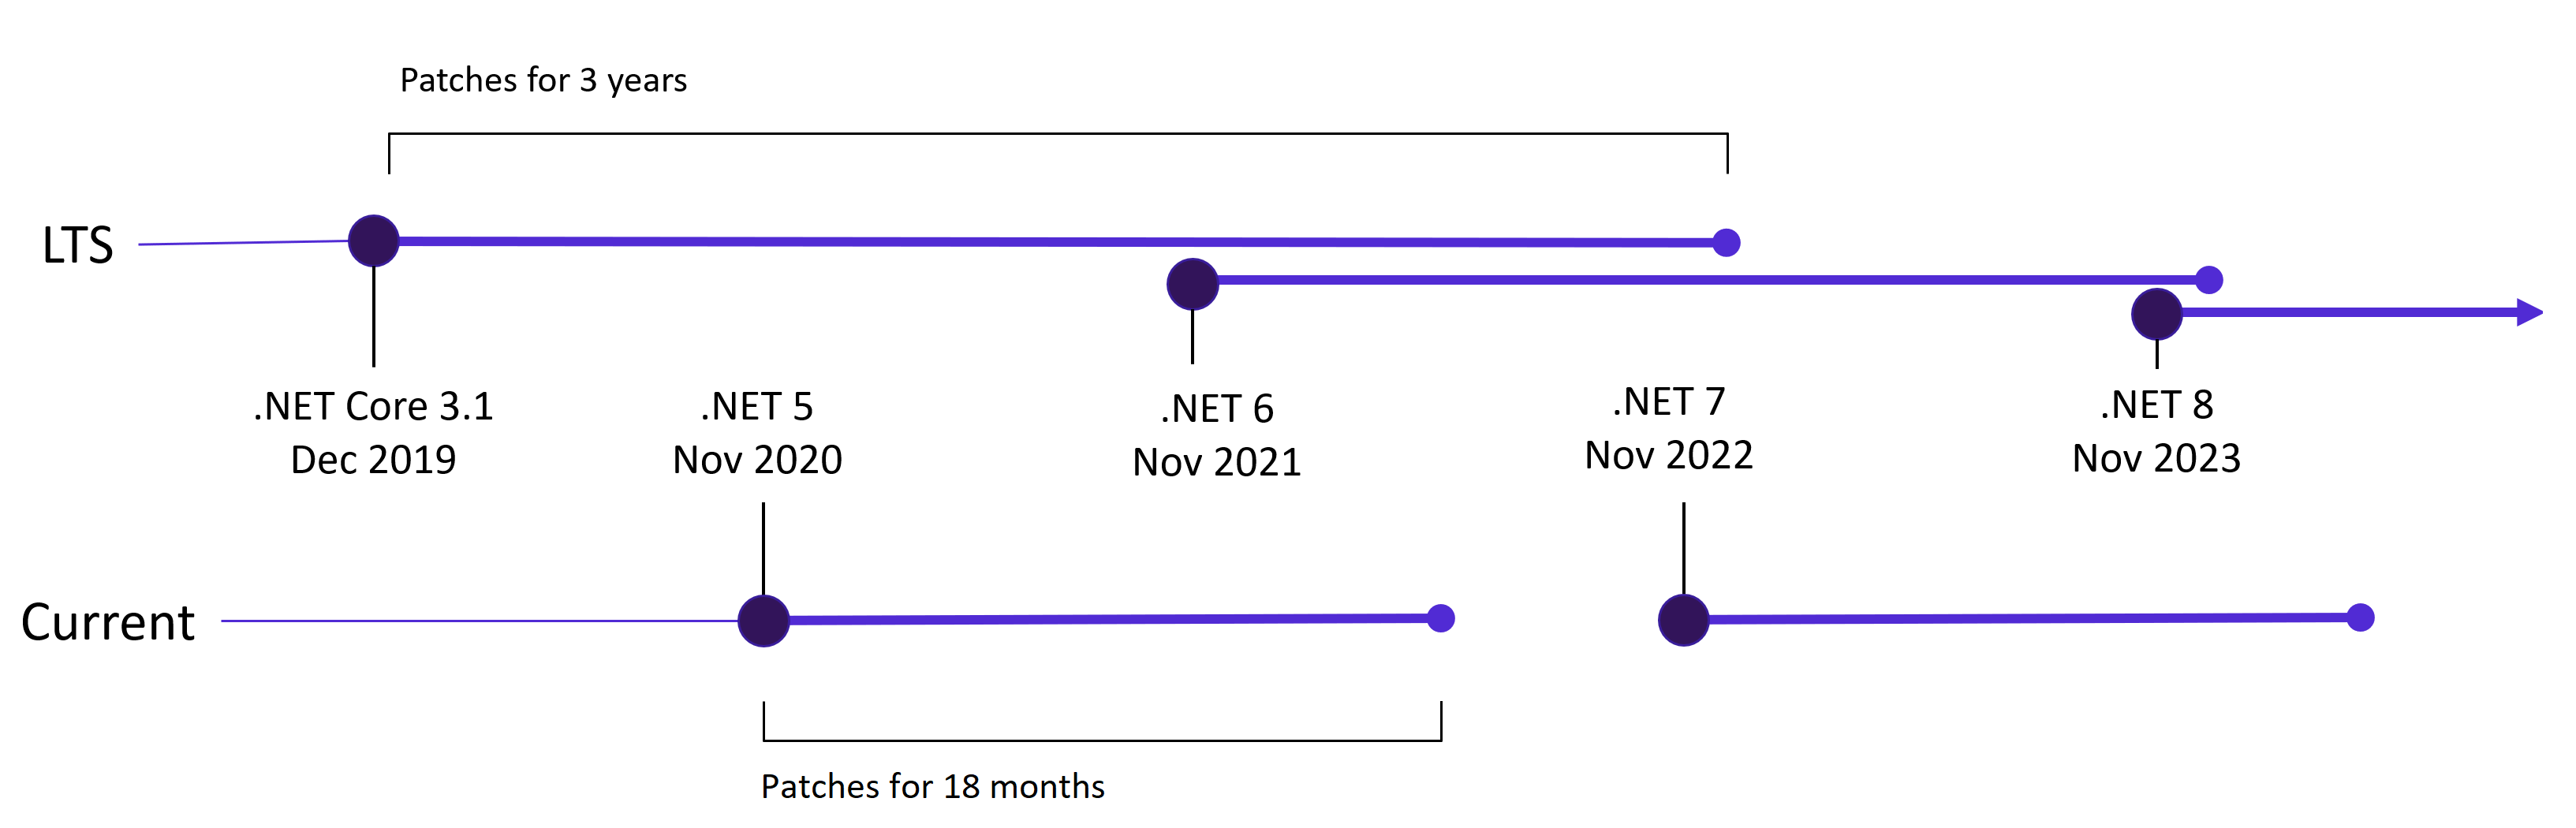
\includegraphics[scale=0.176]{img/dotnet-release-schedule.png}}
    \label{fig:dotnet-release-schedule}
    \source{Retirado de \href{https://dotnet.microsoft.com/en-us/platform/support/policy/dotnet-core}{https://dotnet.microsoft.com/en-us/platform/support/policy/dotnet-core}}
\end{figure}

A Figura \ref{fig:dotnet-release-schedule} demonstra o cronograma de lançamento
de novas versões do .NET, sendo todas a partir do .NET Core 3.1 sendo denominas
apenas de .NET seguido do número da versão. A versão mais recente até a
realização deste trabalho consiste no .NET 6.0, que possui um ecossistema
vasto para o desenvolvimento de aplicações web, em nuvem, desktop, IoT
e mobile.

O .NET 6.0 foi escolhido como plataforma para o desenvolvimento da API do
repositório institucional proposto, por meio da linguagem de programação C\#,
visto que consiste em uma plataforma popular, \emph{open source}, e multi
plataforma, e que possui um grande número de bibliotecas disponíveis
por meio do repositório de pacotes Nuget\footnote{https://www.nuget.org/}.

\subsection{React}

Em tradução direta de \citep[p. 30]{Thakkar:2020}, React ou React.js consiste em uma
biblioteca JavaScript de código aberto, criada em maio de 2013 pelo Facebook,
sendo utilizada para construção de interfaces de usuário.

Dentre suas principais características, o React é declarativo, ou seja,
apenas é necessário criar a camada de visão, e o próprio React irá gerenciar
de forma eficiente os estados da aplicação, renderizando somente os componentes
necessários, e os atualizando quando ocorre alguma mudança de estado, por meio
de uma abordagem de reconciliação denominada \emph{Virtual DOM}. O React
também é baseado em componentes, de forma que cada elemento visual da aplicação
pode ser encapsulado em um componente, que possui seus próprios controles de estado,
e que podem ser reutilizados.

Para realizar a criação de uma página ou componente no React, é utilizado a
sintaxe JSX, que consiste em uma extensão do JavaScript que permite juntar
em um único arquivo a parte lógica da aplicação, ao código que será renderizando em
tela. A sintaxe JSX não é obrigatória, porem é recomendada pelo própria React.

\begin{figure}[H]
    \caption{Exemplo de sintaxe JSX}
    \centering
    \frame{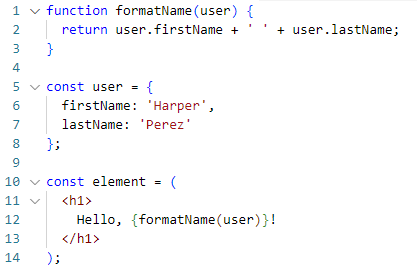
\includegraphics[scale=1]{img/exemple-jsx.png}}
    \label{fig:exemple-jsx}
    \source{Retirado de \href{https://reactjs.org/docs/introducing-jsx.html}{reactjs.org/docs/introducing-jsx.html}}
\end{figure}

A Figura \ref{fig:exemple-jsx} demonstra um exemplo de código em JSX, onde é
utilizado uma função para realizar a formatação de um texto contento um
nome e sobrenome, que será renderizando na interface dentro de uma
tag HTML.

O React foi escolhido como ferramenta para realizar o desenvolvimento da
interface gráfica do repositório institucional proposto, pois é uma biblioteca
gratuita e de código aberto, e extramente popular tanto no mercado de trabalho
quanto no meio acadêmico, além de contar com um vasto ecossistema de bibliotecas
e componentes desenvolvidos pela comunidade.

\subsection{Vite}

Conforme o site oficial da ferramenta \cite{Vite:2022}, o Vite pode ser definido
como sendo uma \emph{build tool} (Ferramenta de Compilação), que possui como objetivo
prover uma experiência de desenvolvimento mais rápida e leve para projetos
\emph{web} modernos, podendo ser utilizado em conjunto a diferentes ferramentas de
desenvolvimento \emph{frontend} como o Vue, React, Preact, Lit, Svelte ou Vanilla.

Dentre os principais diferenciais do Vite, é possível citar a utilização do
\emph{native ES modules} no lugar das tradicionais ferramentas de empacotamento
de código como o Webpack, Rollup ou Parcel. Desta forma o Vite é capaz de
fornecer um ambiente de desenvolvimento com o HMR (\emph{Hot Module Replacement},
que pode ser definido como a capacidade de atualizar elementos visuais em tela
durante o desenvolvimento de uma aplicação, sem a necessidade de recarregar a
página ou recompilar o projeto) extramente rápido, e que tende não ficar lento
com o crescimento da aplicação.

\begin{figure}[H]
    \caption{Exemplo de \emph{dev server} baseado em empacotamento}
    \centering
    \frame{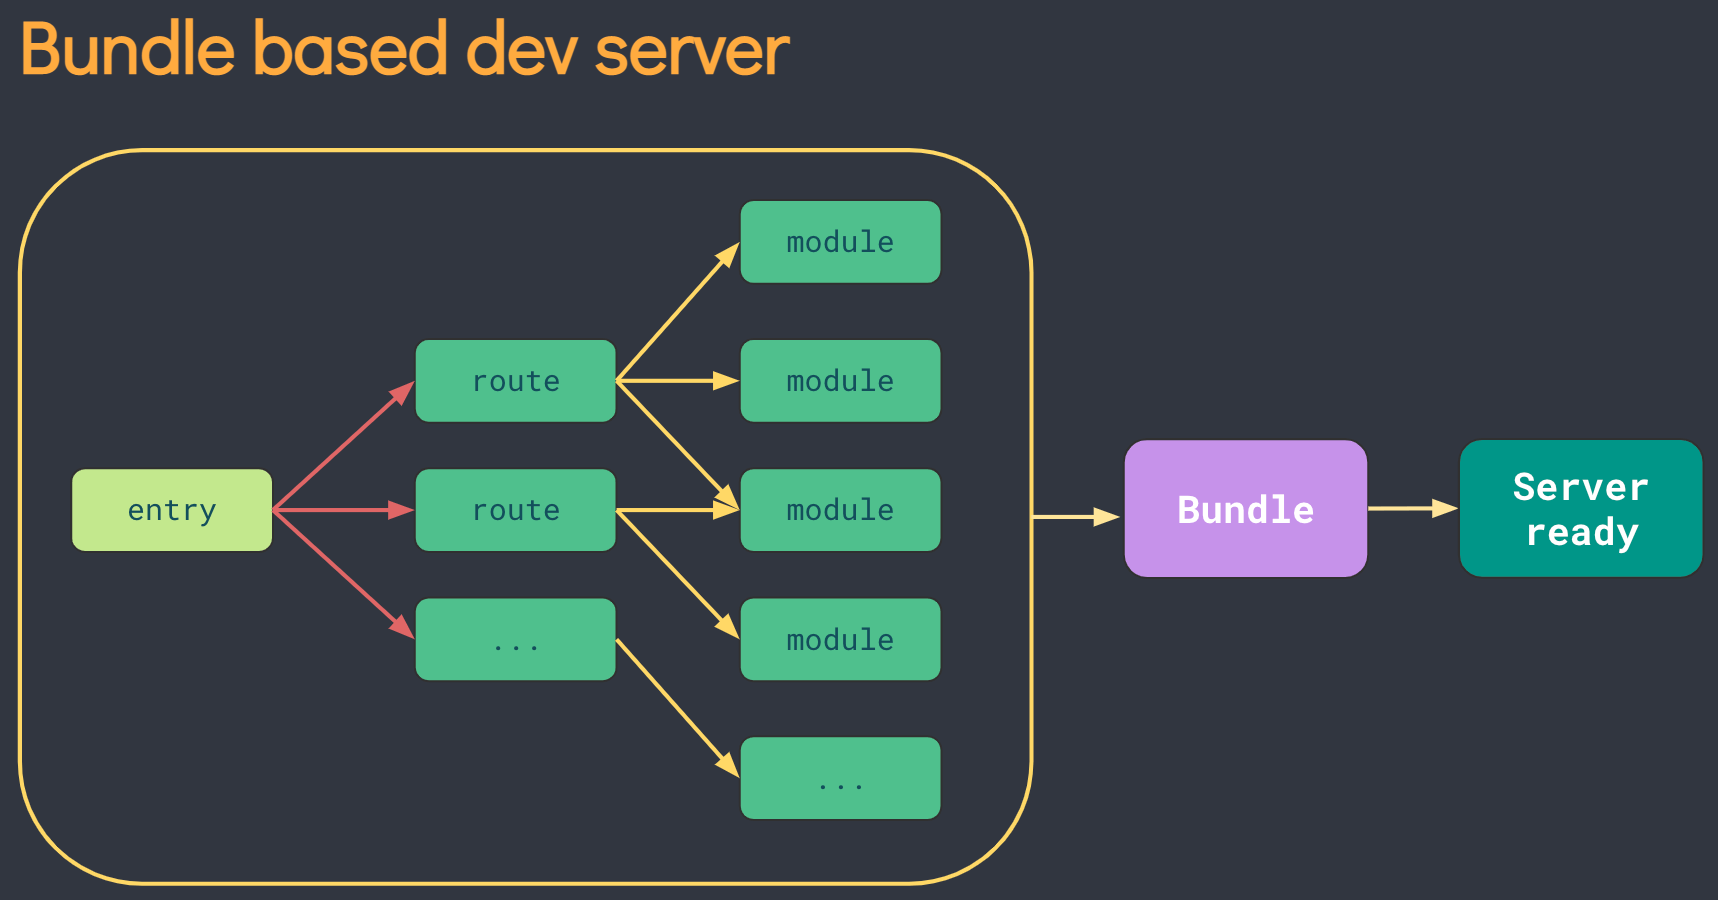
\includegraphics[scale=0.335]{img/bundle-based.png}}
    \label{fig:bundle-based}
    \source{Retirado de \href{https://vitejs.dev/guide/why.html}{vitejs.dev/guide/why.html}}
\end{figure}

Na Figura \ref{fig:bundle-based} é demonstrado o funcionamento de um \emph{dev server}
(servidor de desenvolvimento) baseado no modelo tradicional de empacotamento de código.
Neste é possível verificar que ao realizar a alteração em um arquivo, o \emph{dev server}
ira realizar novamente a compilação de todos os arquivos do projeto para gerar o pacote
de código que será carregado na interface, esta etapa de empacotamento pode levar um tempo
considerável em projetos grandes, onde existem muitos arquivos para serem empacotados.

\begin{figure}[H]
    \caption{Exemplo de \emph{dev server} baseado em \emph{native ES modules}}
    \centering
    \frame{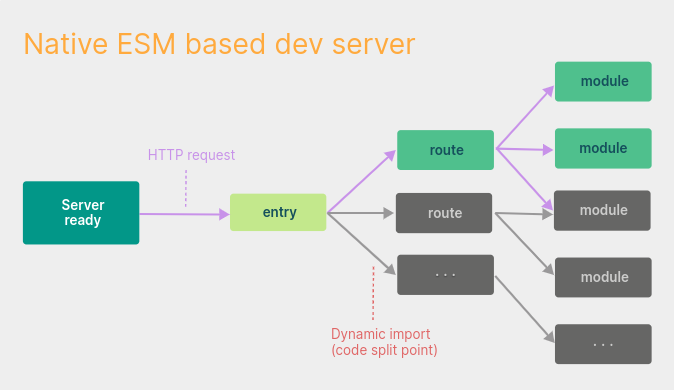
\includegraphics[scale=0.415]{img/esm-based.png}}
    \label{fig:esm-based}
    \source{Retirado de \href{https://vitejs.dev/guide/why.html}{vitejs.dev/guide/why.html}}
\end{figure}

Já a Figura \ref{fig:esm-based} representa o funcionamento de um \emph{dev server}
baseado no modelo de \emph{Native ES Modules}, onde é possível verificar que
não existe uma etapa de empacotamento, o código fonte é fornecido diretamente
ao navegador, que fica responsável por carregar o código a medida do necessário,
realizado a importação de dependências de formas dinâmica para a página que está
sendo exibida.

O Vite foi escolhido como ferramenta de \emph{build tool} para o \emph{frontend}
do repositório institucional proposto, e será utilizada no lugar da \emph{build tool}
padrão do React que utiliza o Webpack para realizar o empacotamento de código,
tendo em vista os benefícios do Vite a longo prazo prevendo o crescimento da aplicação.
Também vale ressaltar que não é necessário realizar adaptações de código especificas
para o Vite, sendo possível trocar para outra ferramenta a qualquer momento sem
grandes dificuldades.

\subsection{PostgreSQL}

Conforme \cite{2017:Carvalho} O PostgreSQL é um Sistema Gerenciador de
Banco de Dados (SGBD) relacional, de código aberto, possuindo a versão 6.0
como sua primeira versão oficial liberada em janeiro de 1997.
Hoje sendo uma alternativa de banco de dados popular, de nível corporativo,
e com mais de 15 anos de desenvolvimento ativo. O PostgreSQL possui uma
arquitetura que entrega confiabilidade, integridade, conformidade a padrões,
desempenho e uma grande quantidade de recursos.

Dentre os seus recursos está o suporte a vários tipos de dados sofisticados,
como o JSON, XML, objetos geométricos e geoespaciais, hierarquias, tags e matrizes.
Além de permitir a inclusão de novos tipos de dados e funções que podem ser
escritas em linguagens suportadas como o SQL, C, Python, Peal, dentre outras.

Como principal recurso que motivou a escolha do PostgreSQL como banco de dados
para o repositório institucional proposto neste trabalho, está o suporte ao
recurso de \emph{full-text search}, que permite uma busca e indexação aprimorada
por textos de grande tamanho na base de dados, que neste contexto será
utilizado para armazenar e indexar os artigos e publicações presentes no repositório.

\subsubsection{Full-Text Search}

Em tradução livre de \cite{2022:PostgreSQL}
o recurso de \emph{Full Text Search} ou Pesquisa Textual Completa,
fornece a capacidade de identificar linguagem natural em documentos
que satisfazem um critério de busca, podendo de forma opcional ordena-los
por relevância aos termos pesquisados. Para realizar este tipo de pesquisa,
são utilizados os conceitos de critério de busca ou \emph{query}, e o
conceito de similaridade. De forma simplificada é possível definir uma
\emph{query} como um conjunto de palavras, e a similaridade como sendo a
frequência que estas palavras sem repetem no documento.

Diferente dos operadores de busca mais comuns presentes em bancos de dados
relacionais como o \emph{like} e \emph{ilike}, o recurso de \emph{Full Text Search}
fornece suporte a um contexto linguístico, permitindo por exemplo, a busca por palavras
derivadas como no caso de \emph{satisfies} e \emph{satisfy} do inglês, algo que
seria extramente difícil de mapear somente com o uso de expressões regulares. Este recurso
também fornece capacidade de indexação para uma pesquisa mais rápida, e ranqueamento
dos resultados para que os resultados mais relevantes apareçam no topo da pesquisa.

Conforme o mesmo autor, para que este tipo de pesquisa seja possível, o texto presente nos documentos precisam
passar por uma etapa de pré-processamento, chamado de extração de dados ou \emph{Tokenization},
onde os textos são convertidos em \emph{tokens} que podem ser separados em diferentes classes,
como palavras, números, endereços de email, etc. Após este processamento, os \emph{tokens}
podem ser convertidos em lexemas ou \emph{lexemes}, que são semelhantes aos \emph{tokens},
porem em um formato normalizado.

Como demonstrado na Figura \ref{fig:ts-vector-exemple} este processo de normalização envolve
deixar todos o texto em minusculo, remoção de sufixos, pluralidade, e em alguns casos até o
gênero das palavras, permitindo que em uma única busca seja possível encontrar por todas as
diferentes variantes de uma palavra. Este processo também elimina as chamadas \emph{stop words},
palavras comuns que não possuem relevância dentro do texto, e que não precisam ser indexadas,
como artigos, preposições, pronomes, conjunções, etc.

\begin{figure}[H]
    \caption{Exemplo de ts\_vector no PostgreSQL}
    \centering
    \frame{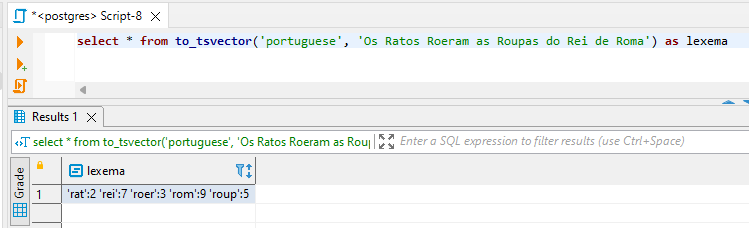
\includegraphics[scale=0.77]{img/ts_vector_exemple.png}}
    \label{fig:ts-vector-exemple}
    \source{Figura do autor}
\end{figure}

No banco de dados PostgreSQL tais lexemas podem ser armazenados utilizando o tipo de
dado denominado de \emph{tsvector}, que possui um conjunto próprio de funcionalidades
para pesquisa textual, sendo o mais comum o operador \emph{@@} que permite a busca por textos
que contemplem um critério de busca, também existe o suporte a pesquisa com operadores lógicos
como \emph{and}, \emph{or} e \emph{not}, e a utilização da função \emph{to\_tsquery} para
converter um texto simples para um \emph{query} de pesquisa.

\subsubsection{GIN Index}

Em tradução livre de \cite{2022:PostgreSQL} o termo GIN consiste em uma
abreviação de \emph{Generalized Inverted Index} ou Índice Generalizado Invertido em
português, também conhecido pelo nome de Lista Invertida, um tipo de índice de banco
de dados projetado para casos onde os items a serem armazenados consistem em valores
compostos, e as pesquisas realizadas devem ser feitas em cada item do conjunto.
Por exemplo, os items a serem armazenados podem ser documentos de texto, e a pesquisa
a ser realizada pode ser feita por documentos que contenham uma palavra em específico.

Conforme o mesmo autor o índice GIN armazena um conjunto de pares de chaves (chave e lista
de ocorrências), onde a lista de ocorrências é um conjuntos de identificadores de linhas
onde a chave/valor foi encontrada. Cada chave é armazenada somete uma única vez,
fazendo com que o índice tenha um tamanho muito compacto, e ao realizar a pesquisa
o índice utilizará o valor chave, no lugar de seu valor real.

Já em tradução de \cite{2011:PostgreSQL}, o índice GIN não apresenta perdas para
grande parte das consultas, porem sua performance depende de forma logarítmica do
número de palavras únicas no texto. Em comparação ao índice GiST (Generalized Search Tree)
que pode ser utilizado por diferentes tipos de dados, o índice GIN apenas pode ser utilizado
em dados do tipo \emph{tsvector}, e alguns quesitos em reação ao desempenho devem ser considerados
ao trabalhar com este tipo de índice.

Como por exemplo segundo o mesmo autor, o índice GIN pode apresentar uma consulta
até 3 vezes mais rápidas que o índice GiST, porem o tempo necessário para sua indexação
pode ser até 3 vezes mais longo. Os indices GIN podem ser mais lentos
de atualizar (cerca de 10 vezes mais lentos do que os índices GiST), se os recursos de
atualização rápida de indices estiverem desabilitados, e o tamanho ocupado pelo índice
GIN pode ser de duas a três vezes maior do que o índice GiST.

O índice do tipo GIN foi escolhido para realizar a indexação do texto das publicações
presentes no repositório institucional proposto, de forma a converter o texto das
publicações em um campo do tipo \emph{tsvector} que pode ser indexado, permitindo
a utilizando das funções de \emph{full-text search} embutidas no banco de dados PostgreSQL
de uma forma rápida e eficiente.

\section{Sistemas Relacionados}\label{sec:rs}
No Quadro \ref{table:related-systems} é apresentado um resumo de sistemas relacionados
a esta pesquisa, contendo o nome do sistema, ano de lançamento, tecnologias,
empresa mantenedora e licença, e site de acesso.

\begin{landscape}
    \begin{table}[H]
        \captionsetup{justification=centering}
        \caption{Sistemas Relacionados}
        \centering
        \label{table:related-systems}
        \setlength\extrarowheight{-1pt}
        \resizebox{1.58\textwidth}{!}{% 
            \begin{tabular}{|p{4cm}|p{2.5cm}|p{4cm}|p{7cm}|p{2cm}|p{7cm}|}
                \hline
                \textbf{Nome}   & \textbf{Lançamento} & \textbf{Tecnologias} & \textbf{Mantenedor}                            & \textbf{Licença} & \textbf{Site}                                                                                      \\ \hline
                Digital Commons & 2004                & Não divulgado        & Elsevier/bepress                               & Comercial        & \href{https://bepress.com/products/digital-commons/}{https://bepress.com/products/digital-commons} \\ \hline
                DSpace          & 2002                & Java e Angular       & DuraSpace/Lyrasis                              & BSD              & \href{https://dspace.lyrasis.org}{https://dspace.lyrasis.org}                                      \\ \hline
                EPrints         & 2000                & Perl                 & University of Southampton                      & GPL 3.0          & \href{https://www.eprints.org/uk}{https://www.eprints.org/uk}                                      \\ \hline
                Islandora       & 2010                & PHP                  & Islandora Foundation                           & GPL 2.0          & \href{https://www.islandora.ca/}{https://www.islandora.ca}                                         \\ \hline
                OPUS 4          & 2010                & PHP                  & Cooperative Library Network Berlin-Brandenburg & GPL              & \href{https://www.opus-repository.org/}{https://www.opus-repository.org}                           \\ \hline
                WEKO            & 2008                & Python e JavaScript  & National Institute of Informatics              & BDS              & \href{https://github.com/RCOSDP/weko}{https://github.com/RCOSDP/weko}                              \\ \hline
            \end{tabular}%
        }
    \end{table}
\end{landscape}

\section{Trabalhos Relacionados}\label{sec:rw}

São apresentados neste tópico, os trabalhos relacionados, que possuem
algum ponto em comum com o que se quer realizar no presente projeto.
Pretendesse aqui, identificar estes pontos, e compará-los com a proposta deste projeto.

\subsection{BDTC - Uma Biblioteca Digital de Trabalhos Científicos com Serviços Integrados}

O trabalho desenvolvido por \cite{2009:Cervi}, possui como premissa a apresentação
de uma proposta de biblioteca digital de trabalhos científicos, que foi denominada como
BDTC, que possui como objetivo prover o suporte a três pontos fundamentais:
auto-arquivamento do conteúdo, extração de metadados e busca de similaridade.

Como um dos principais diferenciais, foi desenvolvido um mecanismo de
busca por similaridade para as pesquisas realizadas na BDTC,
que permite ao usuário encontrar trabalhos relacionados, mesmo que
parte da palavra pesquisada não seja exatamente igual ao conteúdo presente
no documento.

Para o desenvolvimento deste mecanismo de busca, foi utilizado
um recurso denominado \emph{n-gram}, que permite quebrar uma palavra em
conjuntos de letras de tamanhos variados, é retratado como exemplo o
\emph{3-gram} do termo "Juci", que podem ser quebrado em dois conjuntos de 3
letras, ou seja, \emph{"Juc"} e \emph{"uci"}.

Estes conjuntos são armazenados em uma tabela de índices no banco de
dados, de forma que ao realizar uma consulta a partir de uma palavra,
o sistema retorna todos os trabalhos que contenham algum dos conjuntos
de letras que compõem a palavra pesquisada.

Em relação com o presente projeto, pode ser realizado uma comparação com
a forma como o mecanismo de busca foi desenvolvido na BDTC. Ao envés de
utilizar o recurso de \emph{n-gram}, o sistema proposto neste projeto utilizara
o recurso de \emph{tokenization} presente na ferramenta de \emph{Full Text Search} do
banco de dados PostgreSQL, que possui um resultado final semelhante, porem não
idêntico, visto que o \emph{tokenization} remove o gênero das palavras,
os espaços em branco, palavras comuns e palavras que não são consideradas relevantes.

\subsection{Desenvolvimento da nova Biblioteca Digital da Biblioteca Brasiliana USP: Relato de Experiência}

O relato de experiência desenvolvido por \cite{2019:RodrigoMoreira}
apresenta o desenvolvimento da na nova plataforma de Biblioteca Digital da
BBM, a Biblioteca Brasiliana Guita e José Mindlin, em forma de retrospectiva
desde o projeto-piloto, relatando os principais problemas, êxitos
e desafios encontrados durante o desenvolvimento do projeto, que envolvia
a digitalização e desenvolvimento de uma coleção digital para a biblioteca.

A Biblioteca Brasiliana Guita e José Mindlin foi inaugurada em março
de 2013, sendo um órgão e entidade acadêmica da Pró-Reitoria de Cultura
e Extensão da USP (Universidade de São Paulo). Este biblioteca envolve o
projeto Brasiliana USP, que foi iniciado em 2005, e tem como objetivo
abrigar a coleção Brasiliana, doada por José Mindlin. Dentro do escopo
deste projeto, em 2008 é iniciado o projeto-piloto da Biblioteca
Brasiliana Digital, que visa a preservação do acervo e democratização
do acesso ao material.

Para o desenvolvimento da biblioteca digital, foi optado por realizar uma
customização do sistema DSpace, um \emph{software open source} de repositório
digital, com recursos como o Djatoka (servidor de imagens) e visualizadores
de livros como IIPImage e BookReader.

Como principais problemas e êxitos, foi ressaltado a forma como as customizações
foram realizadas no DSpace, sendo muitas delas realizadas diretamente no código fonte
do programa, tornando extramente difícil ou até impossibilitando a atualização
para novas versões da plataforma. Resultado em inconsistências na
visualização dos documentos digitalizados, lentidão do sistema, dentro outros
problemas que vieram a surgir ao longo do tempo.

Além disto, também foi relatado a rotativada das equipes como um fator de impacto
para a continuidade do desenvolvimento da biblioteca, que em sua
maioria era constituída por bolsistas, estagiários e poucos profissionais
terceirizados contratados por tempo determinado. Também foi constatado
que as máquinas digitalizadoras adquiridas para a biblioteca não eram
adequadas para o manuseio dos documentos do acervo, visto que os documentos
eram obras raras, e que necessitavam de diversos cuidados para a preservação
e conversação do material.

Com o tempo parte dos problemas foram resolvidos, sendo até adquirido novas
maquinas digitalizadoras, mais modernas e adequadas para o manuseio do material
bibliográfico.

Comparando o trabalho relacionado com o presente projeto de pesquisa,
é possível ressaltar que o atual projeto não tem como intenção a digitalização
de um acervo físico, porem o sistema DSpace que foi utilizado no trabalho
relacionado foi identificado como um sistema muito popular para o desenvolvimento
de repositórios acadêmicos e bibliotecas digitais de universidades, sendo
possível utilizar a experiência adquirida na implantação desse sistema durante
o desenvolvimento do repositório acadêmico proposto.

\subsection{Classificação facetada: proposta de categorias fundamentais para organizar teses e dissertações em uma biblioteca digital}

O artigo desenvolvido por \cite{2021:Pereira} tem como
proposta a apresentação de categorias fundamentais, baseadas nos trabalhos
do matemático e bibliotecário indiano S. R. Ranganathan e do \emph{Classification Research Group}, que pode ser utilizadas
durante o desenvolvimento de interfaces de navegação facetada de bibliotecas
digitais e repositórios de dissertações e testes.

Neste trabalho é relatado que é comum em bibliotecas digitais de teses
e dissertações, encontrar problemas referente a facilidade de encontrar
e recuperar documentos neles armazenados, visto que a principal forma de
pesquisa tende a ser por um campo textual, onde é possível efetuar buscas
simples, e em alguns casos utilizar a combinação de operadores lógicos, como
\emph{AND}, \emph{OR} e \emph{NOT}, para buscas mais complexas.

Porem esta forma de pesquisa, por meio de um único campo textual,
exige que o usuário possua conhecimento prévio de noções de lógica,
sigla dos cursos, areas e linhas de pesquisa, e que seja capaz de
utilizar essas informações para construir uma busca mais complexa,
geralmente fazendo com que as pesquisas realizadas retornem resultados
vazios, ou não exibam o total potencial de documentos contidos na plataforma,
levando em consideração questões semânticas dos termos utilizados na pequisa.

Desta forma, a abordagem de pequisa facetada permite que o usuário navegue
pela estrutura conceitual das informações armazenadas no repositório, além de
combinar conceitos de diferentes perspectivas ou facetas (janelas ou menus), sendo uma abordagem
de pesquisa mais eficiente, auxiliando o usuário a encontrar o que procura,
de forma visual e intuitiva a partir de palavras chaves modificáveis em um
vocabulário controlado.

Como resultado de sua pesquisa, foram obtidos as seguintes categorias
fundamentais, seguidas de um exemplo: Documento (Trabalho de conclusão), Tipo (Dissertação, Tese);
Curso (Meteorologia); Linha de Pequisa (Sensoriamento);
Tema (Anomalias climáticas); Especialização do tema (Conservação de Energia);
Localização (Oceano Atlântico); e Ano de publicação (2020).

Em relação ao atual projeto de pesquisa, as categorias fundamentais encontradas
no trabalho relacionado poderiam ser utilizadas para a organização dos documentos dentro do repositório
de trabalhos acadêmicos proposto, podendo ser utilizados em recursos de
filtragem das publicações dentro da plataforma.

\subsection{Garantindo acervos para o futuro: Plano de preservação digital para o Repositório Institucional Arca}

A pesquisa realizada por \cite{2020:Queiroz} tem como objetivo
apresentar o desenvolvimento do plano de ação de preservação digital
para o Arca - Repositório Institucional da Fiocruz, visando descrever
as ações necessárias para garantir a preservação dos documentos, bem como
a adoção de padrões, procedimentos e tecnologias que possam ajudar a garantir
a preservação do seu acervo digital para o futuro.

O repositório institucional da Fundação Oswaldo Cruz (Fiocruz) denominado
Arca, foi criado em 2007 e lançado oficialmente como repositório institucional em 2011,
utilizando como o base o \emph{software open source} Dspace, e tendo como intuito
reunir, hospedar, disponibilizar e dar visibilidade a produção intelectual e cultural
produzida na fundação.

Como padrão referência, o artigo cita o \emph{Open Archival Information System}
(OAIS), presente na norma ISO 14721:2003, e adaptado na normal brasileira
NBR 15472:2007. O OAIS define um modelo para configuração e operação
de um repositório digital de documentos confiável, descrevendo como deve funcionar
a estrutura e fluxo das informações, desde a inserção dos documentos digitais e
metadados, até a forma como ocorre o seu armazenamento e acesso.

Dentre as repensabilidades obrigatórias para atender o modelo OAIS
está a documentação das políticas e procedimentos para garantir
a preservação dos documentos a longo prazo, bem como o plano de ação
de sucessão caso o repositório seja desativado ou substituído por outro.

Como resultado de sua pesquisa, foi elaborado uma estrutura básica
do Plano de Ação de Preservação Digital, onde em primeiro momento
é descrito os elementos essenciais para a preservação, como: o cenário
institucional, a descrição da coleção, avaliação de riscos e ameaças,
e o planejamento das estrategias para prevenção de obsolescência. E em
segundo momento, é optado por uma combinação de estrategias de preservação
a serem aplicadas, como a normalização de formatos de arquivos, e a verificação
periódica do formatos dos arquivos em uso, que possam apresentar riscos
de obsolescência tecnológica.

Como contribuição ao atual projeto de pesquisa, pode ser citado a
apresentação ao padrão OAIS, que pode ser utilizado durante o desenvolvimento
do repositório acadêmico, visando a conformidade com padrões internacionais
de desenvolvimento de repositórios acadêmicos confiáveis, além da apresentação
de um plano de ação de preservação digital, que envolve a sucessão das obras
armazenadas em caso de desativação ou substituição do serviço.

\subsection{O mapeamento dos repositórios institucionais brasileiros: perfil e desafios}

O artigo realizado por \cite{2019:Weitzel} tem como objetivo mapear
os repositórios institucionais brasileiros até o período de maio de 2017,
com a finalidade de identificar a atual situação de conformidade com
a estrategia do Acesso Verde Aberto proposto pela BOIA (\emph{Budapest Open Access Initiative}),
além de contribuir com a orientação de diretrizes nacionais e internacionais
para implementação e desenvolvimento de repositórios institucionais, ou sua integração
em rede.

A BOIA (\emph{Budapest Open Access Initiative}) estabelece duas estratégias
de Acesso Aberto, sendo a primeira o Acesso Aberto Dourado, que se baseia
nos esforços da comunidade cientifica para criar um ambiente ideal onde
os periódicos eletrônicos são disponibilizados sem cobrança de assinaturas
ou taxas impostas pelas editoras, como as APCs (\emph{Article Processing Charges}).
A segunda estratégia é o Acesso Aberto Verde, onde o próprio autor
realiza a publicação de seu periódico, seja a versão inicial ou
final, em um repositório institucional.

Para a realização do estudo, foi realizado um levantamento de dados em
fontes como o OpenDOAR, ROARMAP, ROAR, Lista de Repositórios do IBICT,
edital da FINEP, lista de usuários do DSpace e os repositórios listados
no \emph{The Ranking Web of World Repositories}. Como indicador de
alinhamento com o Acesso Aberto Verde, foi realizada a observação
direta sobre cada um dos repositórios, de forma a verificar se o mesmo
disponibiliza o acesso aos artigos de periódicos.

Como resultado, foi constatado que cerca de 54,5\% dos 101 repositórios
analisados estão alinhados com o Acesso Aberto Verde, concentrando 97,5\%
do total de artigos disponíveis em repositórios brasileiros. Também foi
identificado que os sites agregadores de repositórios mundiais não
expressam a realidade, contendo informações mal catalogadas,
\emph{links} quebrados, dentre outros problemas.

Em relação ao atual projeto de pesquisa, é possível citar a contribuição
por meio da apresentação dos conceitos de Acesso Verde Aberto e Acesso
Dourado, que visam disponibilizar os artigos de periódicos em repositórios
institucionais, sem cobrança de taxas ou assinaturas. Também é possível
ressaltar a apresentação de agregadores como OpenDOAR, onde é possível
verificar que majoritariamente os repositórios brasileiros são
desenvolvidos em cima do \emph{software} DSpace.

\subsection{Encontrabilidade da informação no repositório institucional da Unesp: um estudo de eye tracking em dispositivos móveis}

A dissertação de mestrado elaborada por \cite{2019:FernandesMacedes}
possui como objetivo compreender a forma como ocorre a encontrabilidade
da informação em repositórios institucionais a partir do uso de dispositivos
moveis, tendo como base o Repositório Institucional da UNESP.

Para o desenvolvido da pesquisa foi utilizado do método quadripolar, onde
no polo epistemológico foi realizado a definição do objetivo da pesquisa,
no espoco da Ciência da Informação; no polo teórico é realizado a
fundamentação conceitual sobre repositórios digitais, encontrabilidade
da informação e dispositivos moveis; no polo técnico foi utilizado um
conjunto de metodologias com \emph{checklist}, teste com \emph{eye tracking},
e entrevistas; e no polo morfológico é realizado a apresentação dos resultados.

Por meio da pesquisa realizada, foi constatado que grande parte dos
repositórios são criados com base no \emph{software open source} DSpace,
que em suas versões mais recentes já possui uma interface responsiva,
sendo adequada a diferentes tamanhos de telas. Porem, visto que as
atualizações do \emph{software} DSpace dependem da equipe técnica das instituições,
muitos repositórios acadêmicos se encontram desatualizados, tornando
difícil a navegação via dispositivos moveis.

Neste ponto é possível traçar uma correlação ao trabalho desenvolvido por
\cite{2019:RodrigoMoreira}, onde é constatado que as
personalizações realizadas pelas instituições no DSpace,
podem acabar dificultando ou até impedindo a atualização do
\emph{software} para novas versões.

Como resultados de sua pesquisa, foi constatado que o Repositório
Institucional UNESP já possui algum nível de preocupação com a
responsividade para dispositivos moveis em seu \emph{website},
entretanto com a pesquisa realizada foram encontrados alguns
pontos que podem ser aprimorados.

Entre os tópicos que podem ser aprimorados no repositório,
um dos principais seria a falta da caixa de busca no corpo
da página, que se encontra oculto dentro de um menu. A sugestão
seria que esta caixa de busca esteja visível logo no primeiro
momento, pois é um dos elementos principais dentro do repositório.

Sendo assim, foi possível afirmar que no repositório analisado,
elementos não relevantes em dispositivos moveis possuem maior destaque
do que outros elementos que possuem maior importância,
como por exemplo a função de auto-arquivamento,
sendo um recursos muito pouco utilizado a partir de dispositivos moveis,
e que possui uma visibilidade maior que a caixa de pesquisa.

Outros recursos que podem ser aprimorados no repositório seriam
o recurso de autocompletar na caixa de busca, facilitando a localização
dos conteúdos pesquisados. E o recurso de \emph{wayfinding} poderia ser
melhorado, mudando a cor de \emph{links} já visitados, componentes
de \emph{breadcrumb} alternativos para dispositivos moveis, e
\emph{link} visível para retornar a pagina inicial.

Como contribuição ao trabalho atual, é possível ressaltar o resultados
obtidos com a análise de \emph{eye tracking} realizado pela pesquisa,
podendo ser utilizada para a criação de uma interface gráfica para
o repositório acadêmico, que exiba conteúdos mais relevantes para
os usuários de dispositivos moveis.

\subsection{The Emergence of Institutional Repositories: A Conceptual Understanding of Key Issues through Review of Literature}

Na pesquisa realizada por \cite{2018:Saini} é realizado uma revisão de
literatura sobre o surgimento dos repositórios institucionais,
buscando a compreensão conceitual dos principais problemas que envolvem
a criação e uso de repositórios institucionais. A revisão de literatura
consiste em uma organização conceitual da combinação de resultados que provem
contexto para pesquisas. Ajudando a refinar ideias, conhecer especificações do
método de pesquisa, e trazer claridade sobre diversos fatores que cercam o
surgimento, motivação, custos, seleção de \emph{software} e uma perspectiva global
de sobre os repositórios institucionais.

Em sua pesquisa, foi constatado que o surgimento dos repositórios institucionais
não consiste em um fenômeno recente em instituições acadêmicas, e que este tema já vem
existindo por quase uma década, surgindo primeiramente em bibliotecas de instituições
de grande porte, que realizaram o papel de \emph{early adopters} no desenvolvimento
de repositórios institucionais mais focados na acumulação, preservação e disseminação
da pesquisa realizada na instituição, de uma forma acessível e aberta.

Como motivação para a adoção de repositórios institucionais, é considerado
que estes fazem parte da plataforma de serviços oferecidos pela instituição,
sendo um recurso que pode ser utilizado para vender e divulgar o nome da instituição,
de forma a propagar as suas pesquisas e facilitar o intercambio de conhecimento.

Já sobre os fatores de custos, é possível elencar um elevado número de considerações,
como a utilização de \emph{software open source} ou o licenciamento de \emph{software}
proprietário, a abertura de acesso fora do campus, ou o fornecimento de acesso total, ou
limitado do conteúdo. Também foi relatado que dentre os maiores está o custo operacional
da biblioteca, e que ao optar pelo auto arquivamento digital, boa parte dos custos
podem ser evitados.

Sobre a atuação de \emph{softwares open source}, foi relatado que os dois sistemas mais
predominantes são o Eprints e o DSpace. O Eprints foi lançado em 2000, desenvolvido por
Stephen Harnad e sua equipe na Universidade de Southampton, já o DSpace foi lançado 2002
pelo Instituto de Tecnologia do Massachusetts (MIT). O Eprints foi projetado para suportar
formais mais tradicionais de publicações, como periódicos, conferencias, artigos, capítulos
de livros, e outros. Já o DSpace tem como intenção suportar uma variedade muito maior de
documentos, como comunicados formais da instituição, e outras categorias de literatura.

Por fim, sobre a perspectiva global de repositórios institucionais, foi relatado que
a maior parte se encontra na Europa, contribuindo com 47.92\% do total,
seguido pela América do Norte com 29.28\%, Asia com 11.04\%, Austrália com 5.84\%,
a América do Sul com 4.40\%, e Africa com 1.52\% dos repositórios mundiais, tendo como fonte
dados de março de 2018 presentes no OpenDoar.

Este artigo pode ser visto como relacionado, visto que atua como uma revisão de literatura
sobre o surgimento dos repositórios institucionais, que pode ser utilizada como embasamento
para a atual pesquisa, trazendo dados referentes a motivação, custos e \emph{softwares} existes.

\subsection{Why So Many Repositories? Examining the Limitations and Possibilities of The Institutional Repositories (IR) Landscape}

No trabalho realizado por \cite{2018:Arlitsch} possuir como objetivo examinar as limitações
e possibilidades encontradas no cenário de repositórios institucionais. Em sua pesquisa
foi identificado que o número de repositórios vinha crescendo lentamente até meados de 2005,
período em ocorreu um grande aumento no número de repositórios existentes, de 128 em dezembro
de 2005 para 2,253 em dezembro de 2012 conforme dados do OpenDoar, representando um aumento
de 1660\% durante o período.

Todo via, grande parte dos repositórios que surgiram ao longo do tempo são hospedados e
mantidos de forma local pela própria instituição, oque até possui alguns aspectos positivos,
como a flexibilidade, controle, customização, e a tendência de vários sistemas distribuídos
possuírem menor risco de falha massiva que um único sistema centralizado.

Porem também existem aspectos negativos sobre a existência de múltiplas instâncias
de repositórios acadêmicos sendo hospedados em vários locais, por diferentes
instituições, como por exemplo a pesquisa e encontrabilidade do conteúdo, problemas
com a coleta e armazenamento dos metadados, e a variedade de diferentes versões de
\emph{software} sendo utilizadas.

É relatado que a fragmentação da utilização de diferentes versões de \emph{software}
pela comunidade é um tópico dramático, citando como exemplo o \emph{DuraSpace Registry}
que realiza a listam dos repositórios que utilizam como base o DSpace, foi identificado
cerca de 2,004 repositórios que estavam rodando a plataforma DSpace até dezembro
de 2017, destes cerca de 800 (quase 40\%) estavam utilizando a versão 1.8 ou
menor, uma versão lançada em 2011, sendo que qualquer versão abaixo de 5.x não é
mais suportada desde janeiro de 2018.

As implicações negativas desta situação não podem ser ignoradas pelas instituições,
visto que a cada nova versão de \emph{software} que é lançada, fica mais desafiador
para as instituições realizar a atualização destes sistemas. Além da sucessão a
riscos de segurança e ataques de ransomware, que comprometem a confiança que a comunidade
possui em depositar suas publicações nestes repositórios.

Em sua pesquisa é citado que a ideia das instituições hospedarem seu próprio repositório
institucional de forma local já está obsoleta, e deveriam ser substituídos por alternativas viáveis,
fazendo uma relação ao tempo que as instituições também hospedavam os seus próprios servidores de
email, onde hoje em dia são utilizados serviços baseados em nuvem como os fornecidos pela
Google e Microsoft.

Porem o conceito de alternativa viável pode cobrir muitas possibilidades,
e não existe um acordo comum sobre uma escolha correta, algumas discussões focam na adoção de versões
mais recentes de sistemas como o DSpace e Fedora Commons, outros focam em soluções comerciais
baseadas em nuvem, que oferecem escalabilidade e redundância.

Como conclusão, é estimado que a proliferação de repositórios locais por bibliotecas de
instituições acadêmicas, criam mais problemas do que trazem benefícios, considerando
que existem algumas vantagens de possuir um controle local, porem a existência de
centenas de repositórios diferentes não servem mais ao usuário comum, e acabam trazendo
diversos problemas e custos.

Este trabalho pode ser visto como relacionado a presente pesquisa, visto que aborda
tópicos relacionados as vantagens e desvantagens de possuir um repositório local, ou
investir em soluções baseadas em nuvem que podem ser fornecidas como serviços a instituição.

\subsection{Next generation Institutional Repositories: The case of the CUT Institutional Repository KTISIS}

O trabalho relacionado de \cite{2019:Zervas} possui como foco a transformação
do repositório institucional da \emph{Cyprus University of Technology} (CUT) denominado
KTISIS, em um \emph{Current Research Information System} (CRIS), sendo a primeira
apresentação de uma implementação europeia baseada no \emph{software open source}
DSpace-CRIS.

A motivação para a elaboração da pesquisa consiste em atender as necessidades
dos pesquisadores, permitindo que possam submeter seus trabalhos e perfil acadêmico
para o KTISIS. Tendo como alteração do KTISIS mais notável a provisão do Perfil do Acadêmico,
onde os pesquisadores terão acesso dedicado a um conjunto de funcionalidades que
agregam valor aos seus trabalhos, e ao próprio repositório.

Os trabalhos realizados no KTISIS possuem como objetivo seguir as diretrizes e
os comportamentos sugeridos pela \emph{Next Generation Repositories} publicado
pelo COAR (\emph{Confederation of Open Access Repositories}), que visam
colocar os repositórios em posição para a fundação de uma infraestrutura de rede
globalmente distribuída para a comunicação acadêmica.

Como principais benefícios da transformação do repositório KTISIS em um sistema
CRIS usando o DSpace-CRIS, está a provisão de um modelo de dados flexível
que permite descrever todas os documentos que compõem o ambiente acadêmico e suas
ligações, por meio da provisão de identificadores únicos que permitem criar relações
entre os documentos do sistema, como por exemplo o ORCID (\emph{Open Researcher and Contributor ID})
que seria o identificador do pesquisador. Também foi realizado o uso da
funcionalidade que permite importar registros de bases de dados externas
como a Web of Science e o Scopus.

Como contribuição a atual pesquisa, é possível constatar a apresentação dos
conceitos de \emph{Next Generation Repositories} que visa fornecer diretrizes
e sugestões para o desenvolvimento de repositórios acadêmicos preparados
para uma rede global de comunicação acadêmica. Alem dos conceitos de identificadores
únicos para relacionar e citar documentos e autores no repositório como o ORCID.

\subsection{Using Open Access Institutional Repositories to Save the Student Symposium during the COVID-19 Pandemic}

O trabalho relacionado de \cite{2022:Symulevich} tem como objetivo
descrever como duas universidades utilizaram de seus repositórios
institucionais para adaptar os seus simpósios de pesquisa acadêmica
a eventos virtuais em questão de semanas.

O primeiro caso traz o relatado de como a mostra de primavera para pesquisa e
inquérito criativo da universidade de Longwood teve de ser adaptada para um
evento online. A universidade de Longwood consiste em uma universidade publica
do centro-sul da Virginia nos Estados Unidos, que desde a primavera de 2018
realiza um simpósio de pesquisa acadêmica de alunos dos cursos de graduação,
de forma presencial.

Com o crescimento dos casos de COVID-19, os administradores da instituição
começaram a discutir a possibilidade de alterações na forma como os eventos
são realizados, sendo constatado que o repositório acadêmico da universidade
poderia ser utilizado para hospedar as publicações do evento.

Após a aprovação da ideia, o diretório de pesquisas contatou a biblioteca da universidade sobre
a possibilidade da utilização do repositório Bepress Digital Commons\footnote{https://bepress.com/},
para hospedar as publicações do evento virtual, além de requisitar ferramentas
para facilitar a comunicação entre os acadêmicos por meio e de comentários
que são realizados durante a apresentação do evento de tres dias.

Dentre as ferramentas, foram elencados o Disquis\footnote{https://disqus.com/}
e o Intense Debate\footnote{https://intensedebate.com/} como ferramentas para troca
de comentários. Também foram discutidas soluções para o envio de apresentações
no formato PowerPoint que continham videos embutidos, visto que o arquivo do video
é separado do arquivo da apresentação.

A Universidade de Longwood realizou outros dois eventos no formatado virtual,
no outono de 2020 e na primavera de 2021. Os organizadores optaram por migrar
para a plataforma Symposium by Forager One\footnote{https://symposium.foragerone.com/}
para a realização dos eventos.

O segundo caso aborda a realização do simpósio virtual de pesquisa acadêmica
da \emph{University of South Florida St. Petersburg}, sendo uma ramificação
da \emph{University of South Florida} (USF). Com a chegada da COVID-19,
a universidade teve de se adaptar ao ambiente virtual, e pausar as atividades
presenciais no campus. Com isto o escritório de pesquisa começou a entrar em contato
com os bibliotecários da \emph{Nelson Poynter Memorial Library} para discutir
a possibilidade de um simpósio virtual.

Uma variedade de plataformas foram elencadas como candidatas para realizar
a hospedagem do simpósio, como o Website do campus, Canvas, LibGuides,
Bepress Digital Commons, e até o Facebook. Porem levando como critério fatores
relacionados a moderação, segurança, engajamento e arquivamento, foi optado
pela recomendação do próprio repositório da instituição para hospedar o
simpósio virtual.

Como o escritório de pesquisa queria manter uma experiência semelhante
ao evento presencial, foi requisitado que a plataforma incluísse tanto opções
de video quanto de audio, publicação e visualização de posters, e participação
por meio de comentários.

A biblioteca teve de realizar upload de 55 projetos de pesquisa, 43 deles
contendo uma apresentação em audio ou video. Para realizar o upload dos arquivos
foi optado por elaborar uma planilha de metadados como o nome dos autores,
títulos das publicações, abstract's e links para os arquivos de audio e video,
permitindo o upload em massa das publicações de uma única vez.

Como o repositório da instituição era feito em com base no Bepress Digital
Commons, sistema que não possui suporte a troca de comentários, o time de
tecnologias optou por integrar a ferramenta Intense Debate ao repositório
para poder cumprir com o requisito.

Este pesquisa pode ser considera relacionada ao atual trabalho, uma vez
que relata os desafios enfrentados pelas instituições na tentativa de
hospedar seus simpósios virtuais dentro de repositórios institucionais.
Além de citar tecnologias e recursos que foram vistos como necessários
para a realização dos eventos.

\subsection{Understanding Institutional Repository in Higher Learning Institutions: A Systematic Literature Review and Directions for Future Research}

A revisão de literatura desenvolvida por \cite{2019:Asadi} possui como objetivo
proporcionar um melhor entendimento e uma revisão aprofundada sobre o atual estado
dos estudos envolvendo IRs. A pesquisa utiliza o método de revisão sistemática
de literatura e segue um protocolo para organizar de forma apropriada os
trabalhos relatados a repositórios institucionais.

Os dados foram coletados de estudos publicados entre 2007 e 2018, em
seis das maiores bases de dados (ScienceDirect, IEEE Explorer, Springer, ACM,
Taylor and Francis e Emerald Insight), seguindo um critério de revisão, aplicação
a inclusão da pesquisa ou exclusão, com um total de 115 estudos sendo
incluídos na principal parte da pesquisa.

Como resultado da analise dos estudos, foi constatado a falta de conhecimento
sobre repositórios de acesso aberto por escolas e instituições de ensino, e
a infraestrutura inadequada tanto de informação quanto de comunicação, formam
desafios significantes para o desenvolvimento de repositório de acesso aberto.
Também identificado que dentre os maiores benefícios da adotação de repositórios
institucionais estão a visibilidade aumentada da instituição, o aumento em
rankings locais e globais, aumento do prestigio e valor publico, a melhora do
ensino, aprendizado e pesquisa desenvolvida nas instituições.

Também foi relatado que a maior parte dos estudos sobre esta área de pesquisa
focam na ``implantação, implementação e adoção`` e os ``benefícios e desafios``
que tais repositórios trazem as instituições.

Este trabalho de revisão de literatura pode ser considerado relacionado
a atual pesquisa, pois visa trazer embasamento sobre o atual estado
dos repositórios acadêmicos, além de diretrizes para a implementação
de IRs em instituições de ensino.

\subsection{Discovery Tools to Enhance Resources Findability in the Institutional Repositories: an overview}

A pesquisa realizada por \cite{2019:Mettai} possui como objetivo demonstrar
formas como os repositórios institucionais podem melhorar a recuperação e
descoberta por recursos, de forma a melhor suprir as necessidades dos usuários,
por meio da realização de uma analise das interfaces de um conjunto
de repositórios digitais das universidades da Argélia, possuindo como base
a literatura documentada para trazer fundamentação teórica a analise realizada.

Para a realização da pesquisa, foi realizada uma revisão da literatura
envolvendo temas como o surgimento de ferramentas de descoberta, o comportamento
das pesquisas, e validação das ferramentas de pequisa como parte essencial da
biblioteca e repositórios digitais.

No paper é definido uma ferramenta de descoberta (\emph{Discovery Tool}) como
sendo um programa de computador que trabalha como um mecanismo de busca
compreensivo para melhorar a encontrabilidade de recursos, de forma a coletar
todos os metadados de diferentes locais e reuni-los em um único local que
permite pesquisas abrangentes. Também é definido que em geral, estas ferramentas
consistem de dois componentes principais, o primeiro realiza a unificação
e indexação, e o segundo fornece uma camada de descoberta de conteúdo que
provem diferentes recursos como o ranking de relevância, interface intuitiva
e pesquisa facetada.

Em sua revisão de literatura, foi constatado que a maior parte dos usuários
não se sentem confortáveis com a utilização de ferramentas de descoberta de
pesquisa fornecidos por bibliotecas, pois muitos usuários já possuem uma ideia
formada sobre tais ferramentas de pesquisa. Logo quando o Google Scholar
foi lançado, muitos usuários o aderiram de forma imediata, visto que este oferece
uma experiência de pesquisa muito melhor que as interfaces providas por bibliotecas.
Por outro lado, também foi verificado que em geral os usuários se sentem
satisfeitos, e até mesmo preferem utilizar uma base de dados especializada
para temas de pesquisa específicos, ou o Google Scholar para pesquisa de
próstio mais geral.

Em relação ao futuro das ferramentas de descoberta,
é citado 12 recursos que são vistos como essenciais, sendo um local
unificado de pesquisa para toda a informação, uma interface web
que esteja no estado da arte, o enriquecimento de conteúdo, navegação
facetada, campo de pesquisa por palavras chaves em todas as páginas,
ordenação de relevância, mecanismo de correção de texto como ``Você quis dizer...``
e a recomendação de materiais relacionados.

Como contribuição a atual pesquisa, é possível citar os recursos mencionados
como essenciais para ferramentas de descoberta, que também podem ser aplicados
no contexto de repositórios institucionais. Além da apresentação da relevância
de que as pesquisas contidas no repositório devem ser indexadas por mecanismos
como o Google Scholar para ganhar maior visibilidade.

\subsection{Crafting Linked Open Data to Enhance the Discoverability of InstitutionalRepositories on the Web}

O trabalho relacionado de \cite{2019:Jin} realiza um estudo de como o BIBFRAME 2.0
(\emph{Bibliographic Framework}) pode ser utilizado para descrever objetos em repositórios institucionais, tendo como
objetivo trazer esforços conjuntos entre duas comunidades devotadas ao
conhecimento aberto. No estudo é examinado um conjunto de mapeamentos e conversões
do padrão Dublin Core para o BIBFRAME 2.0, para verificar se o novo padrão irá
trazer ganhos na visibilidade dos documentos digitais na web.

No artigo é definido o conceito de \emph{Linked Open Data} como sendo um
método de publicação de dados estruturados, para que estes possam ser
interconectados, de forma a utilizar a rede para conectar pedaços de dados,
informação e  conhecimento dentro da rede semântica (\emph{Semantic Web}), utilizando de URIs e
RDF, normalmente usando de uma licença aberta, que não impeça a utilização
de forma gratuita.

Já o BIBFRAME é delimitado como sendo um modelo de dados para a descrição
bibliográfica, que foi desenvolvido para substituir o padrão MARC, que
era utilizado para acomodar comunidades de usuários amplas como as de museus,
arquivos, e editoras por meio da utilização de princípios de dados conectados,
para tornar os dados bibliográficos mais uteis tanto para a comunidade interna
quanto externa. O BIBFRAME e os conceitos de dados conectados permitem que
os recursos bibliográficos sejam publicados de forma que a \emph{Web} possa
entender, tornando mais fácil encontrar o conteúdo em pesquisas
e buscas realizadas na \emph{Web}.

Para sumarizar o processo de migração, foram extraídas 459 teses do
repositório institucional, após foi realizado a conversão do padrão
Dublin Core para o MARCXML, usando a ferramenta MarcEdit. Em seguida
foi convertido o padrão MARCXML para o BIBFRAME, por meio da ferramenta
\emph{Library of Congress MARCXML to BIBFRAME Transformation software}.

Como conclusão, foram relatados problemas ao realizar a transição do
padrão Dublin Core para o BIBFRAME 2.0, como por exemplo a baixa
qualidade dos metadados no repositório, e outras dificuldades ao
mapear registros entre um modelo e outro, citando que o BIBFRAME 2.0
possui algumas dificuldades em mapear registros não baseados no padrão
MARC.

E possível dizer que este trabalho se relaciona a atual pesquisa, ao
abordar diferentes padrões de armazenamento de metadados que são essenciais
para o desenvolvimento do repositório acadêmico proposto, além de trazer
algumas comparações entre o padrão Dublin Core e o BIBFRAME 2.0.

\subsection{Open Access Scientific Digital Repositories : An Analytical Study of the Open DOAR}

O trabalho relacionado de \cite{2018:Mufazil} possui como principal objetivo
descobrir a composição dos repositórios de dados científicos presentes no
\emph{Directory of Open Access Repositories} (OpenDOAR), baseando-se em
parâmetros como a distribuição regional, contribuição por país, tipo de
repositório, desenvolvimento de coleções, conteudos arquivados,
diversidade de idiomas, \emph{software} utilizado e politicas de metadados.

A pesquisa possui foco no monitoramento do crescimento de OARS
(\emph{Open Access Repositories}) dentre as diversas áreas da ciência
mundialmente registradas no \emph{Directory of Open Access Repositories} (OpenDOAR).
Este iniciado em 2006 pela universidade de Nottingham (UK), consistindo
em um repositório oficial para os OARs, apresentado cerca de 2600 repositórios
no momento em que a pesquisa foi realizada.

Para a realização da pesquisa, foram coletados dados na própria plataforma
do OpenDoar, tendo o espoco da pesquisa limitado somente a repositórios
de pesquisa científica presentes nesta plataforma.

Como resultados, foi revelado que a Europa contribui com o maior número
de repositórios por região, enquanto os Estados Unidos possui a maior
quantidade de repositórios por país. Boa parte dos repositórios analisados
são institucionais, aceitam conteúdo em inglês, reúnem os conteúdos de
periódicos e artigos, alguns possuem coleções, e utilizam o \emph{software}
DSpace para gerenciar o conteúdo, não possuindo policias de metadados
bem definidas.

Em relação ao atual trabalho, e possível citar que a pesquisa se relaciona
ao trazer um contexto geral do estado dos repositórios acadêmicos pelo
mundo, trazendo embasamento sobre tecnologias utilizadas, conteúdos, politicas
de metadados, dentro outros.

\subsection{Evolution of institutional repositories: Managing institutional research output to remove the gap of academic elitism}

O trabalho realizado por \cite{2021:Bashir} possui como premissa realçar a
evolução e estrutura conceitual dos repositórios institucionais, e seus impactos
nos círculos escolar e acadêmico, em termos de melhor visibilidade, aumento
de audiência e comunicação de pesquisa.

O estudo se baseia na examinação
e avaliação vários de periódicos revisados por pares, mostrando inúmeras
dimensões de repositórios institucionais desde sua evolução até aceitação
acadêmica.

Para a realização da pesquisa foi realizada uma revisão de literatura
em bases de dados como Clarivate Analytic’s, Web of Science e Scopus.
Foram utilizados termos como repositórios institucionais, resultado de
pesquisa institucional, repositórios de acesso aberto, acesso aberto verde,
aceso aberto, publicações de acesso aberto, iniciativas de acesso aberto,
bibliotecas digitais, diretório de repositórios de pesquisa aberta,
OpenDOAR, e comunicação escolar.

Como resultado, o estudo revelou que os benefícios associados aos
repositórios institucionais são vários, eles fornecem aos usuários
uma informação que de outro modo estaria indisponível, por razões que
variam entre a falta da disponibilidade de materiais complementares
(como relatórios e papers não publicados, material audio visual,
objetos de aprendizado, referencias bibliográficas, bases de dados,
notas de leitura, dentre outros), a modelos de pagamento ou assinatura
adotados por canais de comunicação escolar.

Também é relatado que a utilização dos IRs está gerando um impacto real
aos modelos de cobrança orquestrados pelas editoras comerciais,
democratizando a voz dos acadêmicos por meio remoção de barreiras
em plataformas estudantis.

Este trabalho pode ser caracterizado como relacionado a atual pesquisa,
visto que aborda questões referentes a como a implementação de repositórios
acadêmicos de acesso aberto podem democratizar o acesso aos materiais de
pesquisa, e remover barrerias impostas pelos valores e assinaturas
cobradas por editoras.

No Quadro \ref{table:related-works} é apresentado um resumo dos trabalhos relacionados citados
nesta pesquisa, contendo o autor, titulo, objetivo, metodologia e resultados
de cada trabalho.

\pagebreak

\begin{landscape}
    \begin{table}[H]
        \captionsetup{justification=centering}
        \caption{Trabalhos Relacionados}
        \label{table:related-works}
        \centering
        \setlength\extrarowheight{-1pt}
        \resizebox{1.58\textwidth}{!}{% 
            \begin{tabular}{|p{5cm}|p{12cm}|p{12cm}|p{4cm}|p{13cm}|}
                \hline
                \textbf{Autor}               & \textbf{Titulo}                                                                                                                           & \textbf{Objetivo}                                                                                                                                           & \textbf{Metodologia}                & \textbf{Resultados}                                                                                                                                                                          \\ \hline
                \cite{2022:Symulevich}       & Using Open Access Institutional Repositories to Save the Student Symposium during the COVID-19 Pandemic                                   & Descrever como duas universidades utilizaram de seus repositórios institucionais para adaptar os seus simpósios a eventos virtuais.                         & Documental                          & Relata os desafios enfrentados pelas instituições na tentativa de hospedar seus simpósios virtuais dentro de repositórios institucionais.                                                    \\ \hline
                \cite{2021:Pereira}          & Classificação facetada: proposta de categorias fundamentais para organizar teses e dissertações em uma biblioteca digital                 & Apresenta categorias fundamentais a serem utilizadas para a construção de uma interface de navegação facetada                                               & Qualitativa e exploratória.         & Foram criadas 8 categorias fundamentais para a navegação facetada.                                                                                                                           \\ \hline
                \cite{2021:Bashir}           & Evolution of institutional repositories: Managing institutional research output to remove the gap of academic elitism                     & Realçar a evolução e estrutura conceitual dos repositórios institucionais, e seus impactos nos círculos escolar e acadêmico.                                & Revisão de literatura               & Foi constatado os benefícios dos repositórios institucionais, e como os IRs de acesso aberto estão democratizando o acesso a pesquisa.                                                       \\ \hline
                \cite{2020:Queiroz}          & Garantindo acervos para o futuro: Plano de preservação digital para o Repositório Institucional Arca                                      & Construção do Plano de Ação de Preservação Digital para o Arca – Repositório Institucional da Fiocruz                                                       & Qualitativa e descritiva            & O Plano de Ação de Preservação Digital do repositório Arca estabelece os padrões que visam garantir que a produção cientifica seja preservada de forma permanente, confiável e segura.       \\ \hline
                \cite{2019:Zervas}           & Next generation Institutional Repositories: The case of the CUT Institutional Repository KTISIS                                           & Documentar a transformação do repositório institucional da \emph{Cyprus University of Technology} denominado KTISIS, em um CRIS.                            & Qualitativa e descritiva            & Foram relatados os principais benéficos da transformação do repositório KTISIS em um sistema CRIS, utilizando o DSpace-CRIS.                                                                 \\ \hline
                \cite{2019:Weitzel}          & O mapeamento dos repositórios institucionais brasileiros: perfil e desafios                                                               & Retratar a situação atual e contribuir com subsídios para orientar as ações e diretrizes para implementação de repositórios.                                & Observação direta.                  & Foi verificado que cerca de 54,5\% dos repositórios concentram 97,5\% do total de artigos dentre os 101 repositórios identificados no país.                                                  \\ \hline
                \cite{2019:RodrigoMoreira}   & Desenvolvimento da nova Biblioteca Digital da Biblioteca Brasiliana USP: Relato de Experiência                                            & Desenvolvimento da na nova plataforma de Biblioteca Digital da BBM (Biblioteca Brasiliana Guita e José Mindlin)                                             & Descritiva e relato de experiência. & Foi optado por realizar uma customização do sistema DSpace, um \emph{software open source} de repositório digital.                                                                           \\ \hline
                \cite{2019:Mettai}           & Discovery Tools to Enhance Resources Findability in the Institutional Repositories: an overview                                           & Demonstrar formas como os repositórios institucionais podem melhorar a recuperação e descoberta por recursos, de forma suprir as necessidades dos usuários. & Revisão de literatura               & Foram ressaltadas questões referentes a utilização de ferramentas de descoberta e pesquisa, e recursos vistos como essenciais nestas ferramentas.                                            \\ \hline
                \cite{2019:Jin}              & Crafting Linked Open Data to Enhance the Discoverability of InstitutionalRepositories on the Web                                          & Realiza um estudo de como o BIBFRAME 2.0 pode ser utilizado para descrever objetos em repositórios institucionais.                                          & Qualitativa e descritiva            & Foram relatados problemas ao realizar a transição do padrão Dublin Core para o BIBFRAME 2.0.                                                                                                 \\ \hline
                \cite{2019:FernandesMacedes} & Encontrabilidade da informação no repositório institucional da Unesp: um estudo de eye tracking em dispositivos móveis                    & Compreender de que forma ocorre a encontrabilidade da informação em repositórios institucionais a partir do uso de dispositivos móveis.                     & Método quadripolar.                 & No repositório analisado elementos não relevantes em dispositivos moveis possuem maior destaque do que outros elementos que possuem maior importância.                                       \\ \hline
                \cite{2019:Asadi}            & Understanding Institutional Repository in Higher Learning Institutions: A Systematic Literature Review and Directions for Future Research & Proporcionar um melhor entendimento e uma revisão aprofundada sobre o atual estado dos estudos envolvendo IRs.                                              & Revisão sistemática de leitura      & Foi constatado que a falta de conhecimento sobre repositórios de acesso aberto e a infraestrutura inadequada formam desafios para o desenvolvimento de repositório de acesso aberto.         \\ \hline
                \cite{2018:Saini}            & The Emergence of Institutional Repositories: A Conceptual Understanding of Key Issues through Review of Literature                        & Buscar a compreensão conceitual dos principais problemas que envolvem a criação e uso de repositórios institucionais.                                       & Revisão de literatura               & Forem levantados dados referentes ao surgimento dos repositórios institucionais, motivação, fatores de custo e \emph{softwares open source}.                                                 \\ \hline
                \cite{2018:Mufazil}          & Open Access Scientific Digital Repositories : An Analytical Study of the Open DOAR                                                        & Descobrir a composição dos repositórios de dados científicos presentes no OpenDOAR.                                                                         & Quantitativo                        & Foram elencados os países com maior numero de contribuição, tecnologias utilizadas, conteúdos armazenados e politicas de metadados.                                                          \\ \hline
                \cite{2018:Arlitsch}         & Why So Many Repositories? Examining the Limitations and Possibilities of The Institutional Repositories (IR) Landscape                    & Examinar as limitações e possibilidades encontradas no cenário de repositórios institucionais.                                                              & Revisão de literatura               & Foi constatado que a existência de centenas de repositórios diferentes não servem mais ao usuário comum, e acabam trazendo diversos problemas e custos.                                      \\ \hline
                \cite{2009:Cervi}            & BDTC - Uma Biblioteca Digital de Trabalhos Científicos com Serviços Integrados                                                            & Apresentação da proposta de biblioteca digital de trabalhos científicos, que foi denominada como BDTC.                                                      & Qualitativa                         & Apresentação uma biblioteca digital de trabalhos científicos que faz uso de serviços como autoarquivamento de conteúdo, extração de metadados dos objetos digitais e busca por similaridade. \\ \hline
            \end{tabular}%
        }
    \end{table}
\end{landscape}
